% paper/wisa2026-en/main.tex
% WISA 2026 camera-ready (LNCS format, up to 12 pages)
% CAMERA-READY TODO before final submission:
%   (1) fill the real author list / affiliations / emails / ORCID iDs below;
%   (2) fill pdfauthor in \hypersetup to match;
%   (3) fill or delete the credits block (acknowledgements / disclosure)
%       before the bibliography;
%   (4) sign the Springer consent-to-publish form (outside LaTeX).

\documentclass[runningheads]{llncs}

\usepackage[T1]{fontenc}
\usepackage{marvosym}% \Letter marker for the corresponding author
\usepackage{graphicx}
\usepackage{amsmath,amssymb}
\usepackage{booktabs}
\usepackage{multirow}
\usepackage[breaklinks=true,hidelinks]{hyperref}
\hypersetup{
  pdftitle={dMIR Peephole Rewrites for Consensus-Critical EVM JITs with First-Class Carry Operators},
  pdfauthor={},% CAMERA-READY TODO: full author list, e.g. First Author and Chunyan Zhao
  pdfsubject={WISA 2026},
  pdfkeywords={Blockchain information systems, EVM JIT, dMIR, Peephole optimization, SMT equivalence checking, Carry chain, Translation validation}
}
\AtBeginDocument{\renewcommand{\doi}[1]{%
  \href{https://doi.org/\detokenize{#1}}{doi:\detokenize{#1}}}}
\usepackage{enumitem}
\usepackage{placeins}
\usepackage{tikz}
\usetikzlibrary{positioning,arrows.meta,calc,patterns}
\usepackage{pgfplots}
\pgfplotsset{compat=1.18}
\setlist[itemize]{topsep=1pt,partopsep=0pt,parsep=0pt,itemsep=0pt,leftmargin=1.4em}
\setlist[enumerate]{topsep=2pt,partopsep=0pt,parsep=1pt,itemsep=1pt}

\begin{document}

\title{dMIR Peephole Rewrites for Consensus-Critical EVM JITs with First-Class Carry Operators}

\titlerunning{dMIR Rewrites for EVM JITs}

% CAMERA-READY TODO: replace every [\,TODO\,] placeholder with the real
% author list (names, order), affiliations, emails, and ORCID iDs.
% Corresponding author: Chunyan Zhao (marked with \Letter).
\author{[First~Author~TODO]\inst{1} \and
Chunyan~Zhao\textsuperscript{(\Letter)}\inst{1}}
\authorrunning{[F. Author TODO] and C. Zhao}
\institute{[Institution TODO], [City, Country TODO]\\
\email{[first.author.email TODO]}, \email{[chunyan.zhao.email TODO]}}

\maketitle

\begin{abstract}
Peephole rewrites in blockchain JIT compilers must preserve transaction semantics bit-for-bit; divergence between consensus-path EVM clients can cause chain forks. Lowering U256 (256-bit) arithmetic to 64-bit hardware creates multi-word carry chains, but LLVM/Alive2 overflow intrinsics expose carry through multi-result tuples, splitting carry-dependent rewrites across SSA nodes. This blocks many rules from direct single-query equivalence checks and leaves engineers to drop them, ship them unverified, or hand-prove them. dMIR, the middle IR of DTVM (an open-source EVM JIT), represents carry and overflow as first-class bit-vector operators, so each dMIR rewrite becomes a single Z3 equivalence query within a two-tier optimization architecture. An offline Z3 admission and coverage pipeline checks all 70 production dMIR rewrites under fixed-width modular bit-vector semantics, including carry-chain rewrites enabled by ADC/SBB operators. A separate x86 CgIR (code-generation IR) layer adds 13 cleanup rewrites validated by matched differential testing rather than SMT. The full 83-rule system achieves a 7.24\% geometric-mean speedup on 27 evmone-bench workloads, with all 5{,}884 paired differential tests across Cancun statetests and EVM-spec unit tests reporting byte-identical final state and matching gas accounting (correctness bounded by suite coverage). This design addresses a verification bottleneck for consensus-critical EVM JITs through a domain-specific IR whose carry and overflow semantics are SMT-checkable.

\keywords{Blockchain information systems \and EVM JIT \and dMIR \and Peephole optimization \and SMT equivalence checking \and Carry chain \and Translation validation}
\end{abstract}

% 01-intro.tex — §1 Introduction
\section{Introduction}

The execution layer of a blockchain information system is a replicated
consensus state machine: every node on the consensus path must produce
bit-identical results for the same transaction. The EVM is a widely
deployed smart-contract execution environment; when a client enables a
JIT, the compiler becomes part of the consensus-critical path.
Peephole rewrites in the JIT act directly during machine-code generation,
so their correctness directly affects the determinism of on-chain
execution; an incorrect equivalence judgment, deployed on only some
clients, may trigger a chain fork.

Existing formal verification of EVM peephole rewrites mostly targets
the block-level bytecode abstraction. The machine-level patterns
emitted by a JIT during code generation---especially the multi-word
carry chains that arise when the 256-bit word size is lowered onto
64-bit hardware---sit at a different abstraction layer from bytecode
rules and are awkward to validate as standard LLVM/Alive2 peephole
queries. The root cause is how IRs model bit-level side results. In
LLVM IR, basic arithmetic is defined only on $N$-bit
integers; the carry bit must be retrieved through an intrinsic that
returns a multi-return tuple of \{result, carry\}. Rules depending on
this carry bit can be expressed only through indirect structures in
Alive~\cite{alive} and similar tools; the bottleneck is the IR's
expressiveness, not the SMT solver~\cite{demoura2008z3}. For a
consensus-critical JIT, an unchecked rule class leaves the engineer
with three choices---drop it (performance), ship it without verification
(safety), or hand-prove it (scalability).

Our approach is to extend the IR with first-class bit-vector operators so
that SMT-checkable peephole rules cover a larger rule class, without
modifying the solver or relaxing the differential-test threshold. In
dMIR, the bit-level patterns that previously required indirect
multi-return encoding are represented directly, so the
corresponding rules fall within Z3 bit-vector equivalence. The SMT scope
is dMIR arithmetic/flag semantics; gas, memory, storage, and x86
equivalence remain outside it.

Concretely, we make three contributions:
\begin{itemize}
\item \textbf{Carry-aware dMIR semantics.} We promote carry and overflow
from implicit side results to first-class dMIR operators, so
ADC/SBB-style multi-word dependencies become single bit-vector
equivalence obligations rather than indirect multi-return encodings.
\item \textbf{SMT admission and production coverage.} An offline Z3
pipeline admits all \textbf{70} production dMIR rewrites under
fixed-width modular bit-vector semantics. Its enumeration also reaches
all production left-hand sides (\textbf{70/70}), including carry-chain
forms that resist direct formulation in LLVM IR.
\item \textbf{Layered optimization with consensus-path evidence.}
SMT-checked dMIR arithmetic simplifications compose with x86-64 CgIR
cleanups validated by matched differential testing; across 27
evmone-bench workloads, the 83-rule system attains a \textbf{+7.24\%}
geometric-mean speedup and passes \textbf{5{,}884} Cancun differential
tests with byte-identical final state and matching gas accounting within
suite coverage.
\end{itemize}

% 02-related.tex — §2 Related Work (drop "and Discussion"; §5.3 limitations removed)
\section{Related Work}
\label{sec:related}

\subsection{Peephole Optimization Frameworks}

{\sloppy
We position our work by abstraction layer, verification method, and
carry-chain coverage. Peephole synthesis and verification frameworks
provide the closest methodological baseline, but they do not by
themselves provide a complete solution for EVM JIT-backend carry
chains. Classical synthesis-then-verification systems include
Denali~\cite{denali_pldi02}, Bansal--Aiken~\cite{bansal_aiken_asplos06},
STOKE~\cite{stoke}, Stratified Synthesis~\cite{stratified}, and
egg~\cite{egg}; SMT-based peephole checking is exemplified by
Alive~\cite{alive}, Alive2~\cite{alive2}, Souper~\cite{souper}, and
PEEK~\cite{peek}; dataflow filtering~\cite{dataflow_pruning} accelerates
search. Recent JIT systems include PyPy's integer-peephole DSL with
build-time Z3 proofs~\cite{pypy_ruleopt} and JOG, which derives Java JIT
optimizations and tests from patterns and detects shadowed optimization
relations~\cite{jog_jit}; LLM-driven LLVM peephole synthesis~\cite{lampo2025}
is a generative complement to deductive enumeration.
We follow the verify-after-enumeration paradigm but move the checked IR
from LLVM IR to dMIR, addressing the multi-return carry and overflow
encoding limit that motivates this paper.\par}

{\sloppy
LeanMLIR~\cite{leanmlir} formalizes IR-parametric peephole verification
in Lean~4, whereas this paper reports a concrete EVM JIT rule set.
Hydra~\cite{hydra} generalizes bit-width-independent rules but, like
Alive2, builds on LLVM IR and inherits the multi-return tuple limit on
the four carry-chain examples in Table~\ref{tab:cannot-express}; closing
that gap via an auxiliary lifted encoding is orthogonal to our
IR-extension contribution. Schett and Nagele~\cite{fmbc20_evm_peephole}
enumerate SMT-checked EVM \emph{bytecode} rules, a higher abstraction
layer than the JIT code-generation path we target with dMIR matching and
x86 cleanup.\par}

\subsection{Verification Work on the Consensus-Critical Path}

Albert et al.~\cite{verified_evm_cav23} give a Coq proof of AOT EVM
bytecode-block rules. Our scope sits at lower abstraction layers: JIT IR
and machine-code, SMT admission at synthesis time, and multi-word carry
chains. Seven rules overlap: 7/83 in our set and 7/14 in their
\texttt{forves} set. This suggests complementary scope rather than a
superset relationship: the remaining 76 cover dMIR algebraic and Boolean
simplifications (including ADC/SBB carry-chain rewrites that motivate
the first-class carry operators) plus 13 x86 cleanup rewrites, none of which are
reachable from the bytecode-block abstraction.

{\sloppy
Runtime divergence detection---Hydra Framework~\cite{hydra_framework},
multi-client detectors, EVM fuzzing, consensus test networks---catches
faults after deployment; our workflow validates rules before deployment.
Bytecode-level EVM
optimization~\cite{maxsmt_evm,vmil24_superinst,ist25_neural_superopt}
is orthogonal to our JIT IR/code-generation focus. Existing work
therefore does not jointly address JIT-backend rewrites, multi-word
carry chains, automated SMT admission, and consensus-critical JIT rewrite validation;
this combination is the gap targeted by our dMIR-based design.\par}

% 03-method.tex — §3 Method
\section{SMT-Checked dMIR Peephole Rewrites}

Offline scripts run Z3 admission and coverage checks over dMIR rule
metadata; the JIT runs a compiled two-tier implementation---dMIR for
algebraic rewrites and x86 CgIR (code-generation IR) for carry-chain
cleanup. The dMIR bit-vector model is in \S\ref{sec:bvmodel}; enumeration
and admission are in \S\ref{sec:synthesis}.

\subsection{dMIR Bit-Vector Semantics and Carry-Chain Operators}
\label{sec:bvmodel}

The core data type of dMIR is a parametric-width bit-vector
$\mathrm{BV}_n$ with $\mathrm{BV}_1$ carrying the carry in/out
($c_{in}, c_{out}$). The carry-propagating addition has signature
$\texttt{ADC}: \mathrm{BV}_n \times \mathrm{BV}_n \times \mathrm{BV}_1
\to \mathrm{BV}_n \times \mathrm{BV}_1$; \texttt{SBB} has analogous
borrow-propagation semantics. In
Z3~\cite{demoura2008z3}, carry propagation zero-extends both 256-bit
operands and the 1-bit carry to 257 bits, sums once, and slices: the
low 256 bits are the result and bit 256 is carry out. This embeds carry
propagation entirely in bit-vector arithmetic with no multi-return tuple
or auxiliary predicate. The model covers dMIR arithmetic and flags; gas,
memory aliasing, storage, and x86 equivalence remain outside it. The same
semantics covers ordinary operators
(\texttt{add}, \texttt{sub}, \texttt{mul}, \texttt{and}, \texttt{or},
\texttt{xor}, shifts); the carry-chain operator is the operator that
general-purpose IRs lack.

\paragraph{Trusted base.} The SMT check assumes the dMIR bit-vector model
agrees with the JIT runtime; the 5884 differential tests of
\S\ref{sec:correctness} show no divergence (random-bytecode fuzzing is
future work, \S\ref{sec:limitations}).

\subsection{Candidate Enumeration and SMT Admission}
\label{sec:synthesis}

\paragraph{Admission check.} For a candidate $\textit{LHS} \to
\textit{RHS}$, we submit to Z3 the proposition $\exists\,\vec{v}.\;
\textit{LHS}(\vec{v}) \neq \textit{RHS}(\vec{v})$. \emph{Unsat} grants
admission under fixed-width modular bit-vector semantics; \emph{sat} or
timeout rejects (sat returns a counterexample). Equivalence assumes
nothing beyond modular arithmetic---no signed interpretation and no
undefined-overflow assumptions. All 70 production dMIR rules pass the
offline Z3 admission check, and CI re-runs this check on every change
to the rule file.

\paragraph{Two enumeration runs.} We report two separate enumeration
experiments with disjoint goals. The \emph{capacity run} fixes a single
grammar---a depth-2 algebraic enumerator plus a small set of
hand-written carry templates---and measures the Z3 admission rate; this
characterizes solver throughput and the typical false-positive boundary.
The \emph{coverage run} extends the same algebraic enumerator with
additional left-hand-side operator tops and a constant-pool widening,
plus a pattern-template instantiation channel reusing the template miner
configuration; this measures whether the tuned offline search space can
reach the 70 hand-designed dMIR production rules, not blind recall on an
unseen rule set. Coverage results appear in \S\ref{sec:evaluation}.

The capacity run uses two complementary paths: \emph{(i) depth-2
algebraic enumeration}---all left/right combinations of depth $\le\!2$
over the dMIR arithmetic and Boolean operators, covering common
algebraic identities; \emph{(ii) carry-template enumeration}---%
multi-word carry-chain candidates constructed by hand around the
carry-chain operators.

\paragraph{Throughput and admission rate.} The capacity run admits
765/775 algebraic candidates (98.7\%, 10 timeouts) and 17/78 carry
templates (21.8\%, 61 semantic rejections): carry-template admission is
limited by 61 semantic rejections, mostly width-mismatch edge cases
(full breakdown in the artifact), while the algebraic side has only 10
timeouts and zero semantic rejections. Full data:
Table~\ref{tab:synth-alive2} (\S\ref{sec:evaluation}). These candidates
measure enumeration capacity; only the curated production rules are
loaded into the JIT at runtime.

\paragraph{Production rule coverage (methodology).} The coverage run
asks a different question: does the enumeration search space contain the
70 hand-designed production dMIR rules? We compare canonicalized
left-hand sides. The \emph{alpha-normalized} canonical form renames
variables to a fixed sequence $x_1, x_2, \ldots$ in traversal order, so
that two rules differing only in operand naming map to the same
representative; commutative pairs (e.g.\ $\texttt{or}(x,y)$ and
$\texttt{or}(y,x)$) likewise collapse to one representative. A
production rule counts as \emph{covered} when at least one
enumerated rule has the same canonical left-hand side; the
\emph{false-miss rate} is the fraction of production rules with no such
match. The match is on canonical left-hand sides only---the enumerated
right-hand side is verified equivalent to the left-hand side by Z3 but
is not required to be syntactically identical to the production
rule's right-hand side. Numerical results appear in
\S\ref{sec:evaluation}.

\paragraph{Counterexamples.} Two rejected carry templates illustrate
why SMT admission is essential on the carry chain.
$\texttt{SBB}(x, x, c_f) \to 0$ fails at $x{=}0, c_f{=}1$ (LHS is
$\texttt{0xFF}\ldots\texttt{F}$; correct form
$\texttt{sub}(0, c_f)$); $\texttt{SBB}(x, 0, c_f) \to \texttt{sub}(0, c_f)$
fails at $x{=}1, c_f{=}0$ (correct form $\texttt{sub}(x, c_f)$). Both
reflect modular-carry traps: ignored carry input and confused operand
polarity. The artifact contains $\sim$2400 lines of Python (enumerator,
template miner, canonical comparator, Z3 admission checks), the rule-set JSON,
coverage output, and unit tests for canonicalization/dedup.

\paragraph{Two-tier rule set.} The dMIR layer handles
machine-independent algebraic simplification (all 70 dMIR rules pass Z3);
the x86 CgIR layer handles hardware-specific cleanup on registers, flags,
and branches (13 syntactic rewrites with \textbf{no separate SMT script},
covered by the matched 5884-test suites of \S\ref{sec:correctness} and
Table~\ref{tab:correctness}). A formal x86 SMT model is future work
(\S\ref{sec:limitations}).

% tables/tab3-1-rule-classes.tex — Two-tier rule classification
\begin{table}[t]
\centering
\caption{Classification of the two-tier peephole rewrite rules by evidence
type. The dMIR rules are checked for equivalence by Z3 on the bit-vector
semantic model; the x86 CgIR rules are covered by matched differential
tests, not by SMT.}
\label{tab:rule-classes}
\footnotesize
\begin{tabular}{@{}l l l r@{}}
\toprule
Layer & Evidence & Category & Count \\
\midrule
\multirow{5}{*}{dMIR} & \multirow{5}{*}{Z3 equivalence check}
  & Boolean normalization  & 42 \\
  & & Algebraic identity     & 15 \\
  & & Identity elimination   & 10 \\
  & & Constant folding       &  2 \\
  & & Dead-code elimination  &  1 \\
\cmidrule(l){3-4}
  & & \textbf{Subtotal}      & \textbf{70} \\
\midrule
\multirow{4}{*}{x86 CgIR} & \multirow{4}{*}{Differential tests}
  & Redundant compare/test cleanup &  8 \\
  & & Branch-fallthrough cleanup     &  2 \\
  & & No-op elimination              &  2 \\
  & & test-setcc merge               &  1 \\
\cmidrule(l){3-4}
  & & \textbf{Subtotal}              & \textbf{13} \\
\midrule
\multicolumn{3}{@{}l}{\textbf{Total}} & \textbf{83} \\
\bottomrule
\end{tabular}
\end{table}


Table~\ref{tab:rule-classes} groups the rules by logical class.
Boolean normalization and algebraic identities together cover most dMIR
rules---these are precisely the patterns the canonical-form enumerator
(\S\ref{sec:synthesis}) is designed to cover. Identity-elimination
and shift-zero patterns admit Z3-discharged proofs in milliseconds,
while the carry-chain class is the one that motivates the operator
extension of \S\ref{sec:bvmodel}.

\paragraph{Selection asymmetry.} The 70 dMIR production rules are
selected manually from recurring profile hotspots and lowering
patterns, then submitted one by one to Z3; this is hotspot-guided
curation, not a claim of systematic optimality. The enumeration pipeline
is a measurement channel: it does not drive production rule maintenance,
and the 1966 admitted candidates are not automatically promoted to
production. The x86-layer rules are covered by code review and matched
test suites. The limitations from this asymmetry are listed in
\S\ref{sec:limitations}.

% 04-evaluation.tex — §4 Evaluation
\section{Evaluation}
\label{sec:evaluation}

\subsection{Enumeration and Admission Output vs.\ the General-Purpose IR}

Table~\ref{tab:synth-alive2} reports the enumeration/admission output
of the capacity run; Alive2's verification on the same rule
sample is summarized below.

% tables/tab4-1-synth-alive2.tex — Synthesis pipeline output with Alive2 comparison
\begin{table}[t]
\centering
\caption{Output of the synthesis pipeline: candidate counts, Z3 passes,
rejections, and admission rate. The two enumeration paths are described
in detail in \S\ref{sec:synthesis}.}
\label{tab:synth-alive2}
\footnotesize
\begin{tabular}{@{}lrrrr@{}}
\toprule
Candidate source & Input & Pass & Reject & Admission rate \\
\midrule
Algebraic enumeration & 775 & 765 & 10$^*$             & 98.7\% \\
Carry templates       &  78 &  17 & 61\phantom{$^*$}   & 21.8\% \\
\bottomrule
\end{tabular}
\vspace{2pt}
\par\noindent{\scriptsize $^*$\,10 candidates returned neither sat nor
unsat within the time limit and are conservatively rejected.}
\end{table}


Z3 discharges the hardest 256-bit queries in $\sim$60\,ms and rechecks
all 70 dMIR rules in $\sim$0.5\,s, so width is not the bottleneck. On a
10-rule U256 capacity-run sample, Alive2 clears the 6 without
multi-return carry but reports type mismatch or timeout on the 4
\texttt{adc}/\texttt{sbb} cases. This sample is separate from the four
production-style cases in Table~\ref{tab:cannot-express}; both expose
the same tuple cause.

\paragraph{Production rule coverage.} Using the canonical-LHS
methodology, the coverage run produces
\textbf{1966} Z3-admitted rewrite rules: \textbf{1856} from the
extended algebraic enumerator and \textbf{110} from pattern-template
instantiation. The pattern-template path starts from 2964 pattern-template candidates,
which Z3 verification and deduplication against the enumerator output
and the existing rule file reduce to the final 110. On the 70
hand-designed production rules, the run matches \textbf{69/69} unique
canonical patterns---one commutative-twin pair, $\texttt{or}(x,y)$
versus $\texttt{or}(y,x)$, shares a single canonical representative
that both production names match---equivalently \textbf{70/70}
production rule names; the false-miss rate against the production set
is therefore \textbf{0/70}.

\paragraph{Scope of the coverage claim.}
\label{sec:coverage-scope}
The claim has two boundaries. First, the result measures coverage of the
\emph{existing} production rule set; the extended enumerator's
left-hand-side operator tops and constant pool were broadened in light
of an earlier 0/70 baseline that exposed mechanical gaps (missing tops
such as \texttt{not}/\texttt{select}/\texttt{shl}/\texttt{ushr}/%
\texttt{sshr} as left-hand-side roots, missing small constants, and
structural-equality dedup of forms such as $\texttt{and}(x,x)$).
Reaching 70/70 therefore demonstrates that the production rules lie
inside an enumerable and Z3-discharged search space; it does not
demonstrate blind recall of an unseen target. Second, coverage is
defined on canonical left-hand sides; the enumerated right-hand side
is verified equivalent to its own left-hand side by Z3 but is not
required to be syntactically identical to the production rule's
right-hand side. Together with the admission rate above, this result
shows the tuned search space is broad enough to contain every
hand-designed rule, while 1966 of its members pass Z3 verification; it
does not claim that the non-production members are useful runtime
rewrites.

\subsection{End-to-End Performance}
\label{sec:perf}

\paragraph{Setup.} Intel Core Ultra 7 265K/Ubuntu 22.04; evmone-bench,
baseline (upstream \texttt{main}) vs.\ rules-enabled side, 20 runs
(30 if CV $\geq3\%$), bootstrap CIs ($B{=}10\,000$), pinned CPU,
turbo off.

% Auto-generated by csv_to_tikz_bar.py — do not edit
\begin{figure*}[t]
\centering
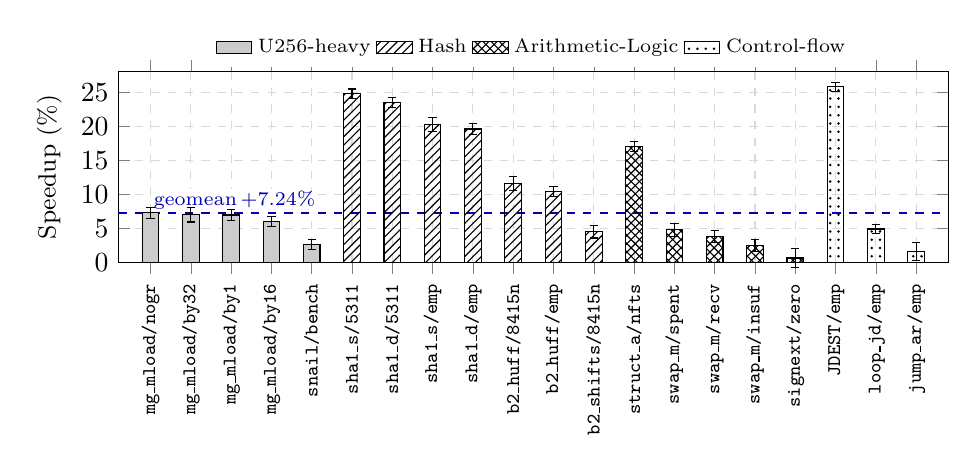
\begin{tikzpicture}
\begin{axis}[
  width=\textwidth,
  height=4.0cm,
  ybar,
  bar width=6pt,
  xtick={0,...,19},
  xticklabels={
    {mg\_mload/nogr},
    {mg\_mload/by32},
    {mg\_mload/by1},
    {mg\_mload/by16},
    {snail/bench},
    {sha1\_s/5311},
    {sha1\_d/5311},
    {sha1\_s/emp},
    {sha1\_d/emp},
    {b2\_huff/8415n},
    {b2\_huff/emp},
    {b2\_shifts/8415n},
    {struct\_a/nfts},
    {swap\_m/spent},
    {swap\_m/recv},
    {swap\_m/insuf},
    {signext/zero},
    {JDEST/emp},
    {loop\_jd/emp},
    {jump\_ar/emp}
  },
  xticklabel style={rotate=45, anchor=east, font=\scriptsize\ttfamily},
  x tick label style={rotate=45, anchor=east},
  ylabel={Speedup (\%)},
  ylabel style={font=\small},
  ymin=0,
  ymax=28,
  xmin=-0.8,
  xmax=19.8,
  ytick={0,5,10,15,20,25},
  grid=major,
  grid style={dashed, gray!30},
  legend style={
    at={(0.5,1.02)},
    anchor=south,
    legend columns=4,
    font=\scriptsize,
    draw=none,
  },
  legend image code/.code={%
    \draw[#1] (0cm,-0.08cm) rectangle (0.45cm,0.08cm);%
  },
  clip=false,
]

% zero reference line
\draw[black, thin] (axis cs:-0.8,0) -- (axis cs:19.8,0);

% geometric-mean reference line (+7.24%)
\draw[blue!70!black, dashed, thick] (axis cs:-0.8,7.24) -- (axis cs:19.8,7.24);
\node[blue!70!black, font=\scriptsize, anchor=south west, fill=white, inner sep=1pt]
  at (axis cs:0,7.24) {geomean\,+7.24\%};

% group: U256-heavy
\addplot[fill=black!20, draw=black, bar shift=0pt, error bars/.cd, y dir=both, y explicit, error bar style={thin}, error mark options={rotate=90, mark size=1.5pt}]
  table[x=x, y=y, y error minus=ym, y error plus=yp] {
    x y ym yp
    0 7.2549 0.8283 0.8210
    1 6.9940 1.0760 1.0637
    2 6.9362 0.7959 0.7892
    3 6.0337 0.7583 0.7522
    4 2.6203 0.7584 0.7526
  };
\addlegendentry{U256-heavy}

% group: Hash
\addplot[pattern=north east lines, draw=black, bar shift=0pt, error bars/.cd, y dir=both, y explicit, error bar style={thin}, error mark options={rotate=90, mark size=1.5pt}]
  table[x=x, y=y, y error minus=ym, y error plus=yp] {
    x y ym yp
    5 24.8066 0.6719 0.6660
    6 23.5105 0.7462 0.7390
    7 20.2360 1.0368 1.0235
    8 19.5875 0.7839 0.7763
    9 11.5442 1.0606 1.0481
    10 10.4090 0.7829 0.7761
    11 4.4577 0.8946 0.8863
  };
\addlegendentry{Hash}

% group: Algorithmic
\addplot[pattern=crosshatch, draw=black, bar shift=0pt, error bars/.cd, y dir=both, y explicit, error bar style={thin}, error mark options={rotate=90, mark size=1.5pt}]
  table[x=x, y=y, y error minus=ym, y error plus=yp] {
    x y ym yp
    12 17.0420 0.7116 0.7056
    13 4.7468 0.9761 0.9662
    14 3.8131 0.9158 0.9072
    15 2.4458 0.9211 0.9124
    16 0.6157 1.3616 1.3432
  };
\addlegendentry{Arithmetic-Logic}

% group: Control-flow
\addplot[pattern=dots, draw=black, bar shift=0pt, error bars/.cd, y dir=both, y explicit, error bar style={thin}, error mark options={rotate=90, mark size=1.5pt}]
  table[x=x, y=y, y error minus=ym, y error plus=yp] {
    x y ym yp
    17 25.7880 0.6690 0.6630
    18 4.8763 0.6924 0.6873
    19 1.5885 1.2836 1.2671
  };
\addlegendentry{Control-flow}

\end{axis}
\end{tikzpicture}
\par\vspace{-4pt}
{\scriptsize \emph{Labels:} mg=\texttt{memory\_grow}, b2=\texttt{blake2b}, sha1\_s=\texttt{sha1\_shifts}, sha1\_d=\texttt{sha1\_divs}, struct\_a=\texttt{struct\_array}, swap\_m=\texttt{swap\_method}, signext=\texttt{signextend}, JDEST=\texttt{JUMPDEST\_n0}, loop\_jd=\texttt{loop\_jumpdest}, jump\_ar=\texttt{jump\_around}, snail=\texttt{snailtracer}.}
\vspace{-4pt}
\caption{Positive-speedup benchmark configurations from enabling the
peephole rewrite rule set over the upstream-main baseline (error bars
are 95\% bootstrap confidence intervals, $B{=}10\,000$). The horizontal
line at zero marks the no-change baseline; the dashed line at
\textbf{+7.24\%} marks the 27-benchmark geometric-mean speedup. From
left to right, the benchmarks are grouped into four workload clusters:
U256-heavy, Hash, Arithmetic-Logic, and Control-flow.}
\label{fig:speedup}
\end{figure*}


{\sloppy
Across all 27 benchmarks, the full 83-rule set improves the geometric
mean by \textbf{+7.24\%} (95\% CI [+2.59\%, +12.11\%]); the
positive-speedup cases are shown in Figure~\ref{fig:speedup}. Peak
speedup is \textbf{+25.79\%} on
\texttt{JUMPDEST\_n0/}\allowbreak\texttt{empty}. The \texttt{sha1}
family gains +19.59\%--+24.81\%, and
\texttt{blake2b\_}\allowbreak\texttt{huff} gains +10.41\%--+11.54\%.\par}
\noindent
Hit rate and speedup are decoupled: \texttt{mg\_mload} matches nearly
every U256 instruction yet gains under 8\%, while sha1 hits only 7.5\%
of opcodes yet gains over 20\% from x86 branch and compare-merge
cleanup. The two layers complement each other: multi-word rules
concentrate gains on U256-heavy contracts, x86 cleanup yields broader
gains on ordinary code.

\paragraph{Compilation overhead.} Across 776 JIT unit-test modules,
median per-module compile time is 0.45\,ms (p95 0.87\,ms) covering the
full loading--analysis--codegen pipeline; this is an upper bound on
the whole pipeline rather than the incremental rewrite-pass cost
(per-pass attribution remains future work).

\subsection{Correctness and Rule Coverage}
\label{sec:correctness}

% tables/tab4-3-correctness.tex — Correctness and rule coverage
\begin{table}[!htbp]
\centering
\caption{Differential test results for the rules-enabled build
(83 added rules) and upstream-main baseline: passes/total.}
\label{tab:correctness}
\footnotesize
\setlength{\tabcolsep}{3pt}
\begin{tabular}{@{}l c c p{2.6cm}@{}}
\toprule
Test dimension & Enabled & Baseline & Suite source \\
\midrule
Unit (JIT)              & 223/223   & 223/223   & EVM spec subset \\
Unit (interpreter)      & 215/215   & 215/215   & Run list \\
statetest (JIT)         & 2723/2723 & 2723/2723 & Cancun 101 suites \\
statetest (interpreter) & 2723/2723 & 2723/2723 & Cancun 101 suites \\
\midrule
Total & \textbf{5884/5884} & \textbf{5884/5884} & --- \\
\bottomrule
\end{tabular}
\end{table}


{\sloppy
Both sides agree item-by-item across the four differential categories of
Table~\ref{tab:correctness} (5884/5884 total). Independently,
\texttt{evmone-statetest} on the Cancun fork reaches the same matrix
under multipass JIT and interpreter modes.\footnote{Cancun is selected
via \texttt{evmone-statetest -k fork\_Cancun}; Prague tests are excluded
because DTVM does not yet support that fork.} The suite covers Cancun
state tests and EVM unit tests, but we do not claim opcode- or gas-branch
coverage completeness.\par}

CI re-runs the same admission check on every change to the rule file;
the timing is distinct from the per-module JIT compile time reported
above.

\FloatBarrier
% 06-conclusion.tex — §6 Conclusion
\section{Conclusion}

This paper builds a two-tier EVM JIT peephole system: 70 dMIR rules pass
Z3 checks over arithmetic and flags, while 13 x86 cleanup rules are
covered by differential runs. First-class carry and overflow operators
let a domain IR cover cases that bytecode-level identities alone cannot.
Future work covers two fronts. On verification, a formal x86 model would
replace the differential-test fallback for the x86 layer, and a complete
Alive2 classification would tighten the comparison with the LLVM IR
baseline. On systems, cross-engine baselines (e.g.\ evmone, revm),
dataflow pruning of the enumeration search, and composition with
bytecode-level rule sets are natural extensions.

% 07-availability.tex — §7 Data and code availability
\phantomsection
\label{sec:availability}
\section*{Data and Code Availability}

Rule sets, Z3 admission checks, evaluation scripts, and data are available
from an anonymous repository upon request to the program chairs and will be
de-anonymized upon acceptance. CI runs the production dMIR validation tests
on every rule-file change.


% CAMERA-READY TODO: fill in (or delete) the credits block below.
% llncs v2.24 provides \begin{credits} with \ackname / \discintname.
%\begin{credits}
%\subsubsection{\ackname} [Funding sources and thanks TODO.]
%\subsubsection{\discintname} The authors have no competing interests to
%declare that are relevant to the content of this article.
%\end{credits}

\bibliographystyle{splncs04}
\bibliography{references}

\end{document}
